% Configuración del tipo páginas
        \documentclass[12pt, a4paper,english,spanish]{amsart}
        \parindent = 10 pt
        \parskip=1.5pt 
        \usepackage[width=15.5cm, left=3cm, top=2.5cm, height= 24.5cm]{geometry}

% Paquete para reconocer la separación en sílabas en español
        \usepackage[utf8]{inputenc}
        \usepackage[spanish]{babel}

% Paquetes especiales
        \usepackage{amsmath}
        \usepackage{amsfonts}
        \usepackage{amssymb}
        \usepackage{upgreek}
        \usepackage{ifthen}
        \usepackage{alltt}
        \usepackage[pdftex]{graphicx}
        \usepackage{subfig}
        \usepackage{float}
        \usepackage{mathtools}
        \usepackage{amsthm}
        \usepackage[vlined,tworuled,commentsnumbered,linesnumbered]{algorithm2e}
        
\begin{document}

\begin{center}
   \Large\textbf{Trabajo practico}\\
   \Large\textbf{Trabajo practico. Probabilidad y Estadistica (C)}\\
   \large\textit{Alejandro Martín Ventura}\\
   \large\textit{249/11}
\end{center}


\begin{section}{Ejercicio 1}
~\\


Sean $X_1, ... ,X_n$ una muestra aleatoria con distribución $U(0, b)$ con b un parámetro desconocido. Calcular analíticamente los estimadores de momentos $\hat{b}_{mom}$ y de máxima verosimilitud $\hat{b}_{mv}$. Implementarlos en R como funciones.


\begin{subsection}{Estimador de momentos}
~\\

Comenzaremos calculando la esperanza de una variable uniforme de parámetros 0 y b.\\
$E(U) = \frac{b+0}{2} = \frac{b}{2}.$\\
~\\

Ahora para la esperanza muestral, obtenemos\\
~\\

$\frac{X_1+ ... +X_n}{n}$. \\
~\\
Igualamos.\\
~\\

  $\frac{X_1+ ... +X_n}{n} = \frac{b}{2}$\\
 $2\frac{X_1+ ... +X_n}{n} = \hat{b}_{mom}$\\
\end{subsection}

\begin{subsection}{Estimador de máxima verosimilitud}
~\\

Tomo $f(X_1, ... ,X_n) = \prod_{i=1}^{n}{f(x_i)} = $ 
$\prod_{i=1}^{n}{\frac{1}{b} I_{[0,b]}(x_i)}$ \\
~\\

Con lo cual se obtiene la siguiente función de verosimilitud:\\
~\\

$L(b) = \frac{1}{b^n} \prod_{i=1}^{n}{ I_{[0,b]}(x_i)}$\\
~\\

Notemos que la función también se puede definir como $\frac{1}{b^n}$ si $0 < X_i < b$ $ \forall i$, o cero fuera de ese rango. O sea, si algún $X_i$ es mayor a b, la función se vuelve nula. \\
Pero esta condición, $0 \leq X_i \leq b$ $ \forall i$ puede pensarse como $ b > max(X_i)$.\\
~\\

Dado que donde no es nula, la función es monótona decreciente, puesto que esta compuesta por un cociente con un denominador positivo y monótono creciente, el máximo debe encontrarse exactamente en el punto en el cual deja de ser nula. Esto es, $max(X_i)$, y por lo tanto, este es el estimador de máxima verosimilitud.\\
~\\

$\hat{b}_{mv} = max(x_i)$
~\\

\end{subsection}


\end{section}



\newpage

\begin{section}{Ejercicio 2}
Implemente el siguiente estimador de b:

$\hat{b}_{med} = 2xmediana\{x_1, ... ,X_n	\}$



\begin{subsection}{Implementación}~\\

Llamare a la función que implementa el estimador pedido, ``Bmed''. A continuación se encuentra el código fuente de la misma.
\begin{verbatim}
Bmed<-function(X)
{
	sX = sort(X)
	n = length(X)
    median = X[n/2]
  return(2*median)
}
\end{verbatim}

Este código define una función que toma un vector X de números y calcula su mediana, luego retorna el doble de la mediana como resultado. Dado que el doble de la media es la expresión del estimador, es una implementación correcta del mismo.


\end{subsection}
\end{section}


\newpage




\begin{section}{Ejercicio 3}
Utilizando $b = 1$, genere una muestra de tama;o $n = 15$. Calcule cada uno de los estimadores con la muestra obtenida y reportar el valor de cada estimador y su error.

\begin{subsection}{Implementacion}
Comenzaremos implementando, como funcion, los dos estimadores restantes.


\begin{verbatim}
Bmom<-function(X)
{
mean = 0
  for(i in 1:length(X))
    { 
      mean = mean + X[i];
    }
    mean = mean/length(X)
  return(2*mean)
}



Bmv<-function(X)
{
  return(max(X))
}
\end{verbatim}


Bmom es la forma algoritmica en R de la expresion del estimador calculado en el primer punto, mientras que la funcion nativa de R, max, nos provee de una forma facil para calcular el estimador Bmv. Se la deja aun asi dentro de una funcion por consistencia.\\
\\
A continuacion se muestra un ejemplo de una corrida en la cual se utiliza la funcion runif, nativa de R, la cual genera numeros flotantes aleatorios siguiendo una distribucion uniforme, para generar la muestra. Luego de eso realiza  la estimacion de b mediante Bmom, Bmv y Bmed.


\begin{verbatim}

> X = runif(15, 0.0, 1.0)
> X
 [1] 0.85100376 0.35369725 0.37211795 0.02894966 0.80028852
     0.73197841 0.24412642 0.84706643 0.74270632 0.85146423
     0.65617966 0.11617666 0.11925780 0.25546167 0.53364961
> Bmed(X)
[1] 0.7442359
> Bmv(X)
[1] 0.8514642
> Bmom(X)
[1] 1.00055


\end{verbatim}

Utilizaremos ahora R para calcular tambien los errores

\begin{verbatim}
> abs(1-Bmom(X))
[1] 0.0005499117
> abs(1-Bmv(X))
[1] 0.1485358
> abs(1-Bmed(X))
[1] 0.2557641
> 
\end{verbatim}

Como puede verse, los valores obtenidos por los estimadores Bmv, Bmom y Bmed son 0.8514642, 1.00055 y 0.7442359 respectivamente, y sus errores son 0.1485358, 0.0005499117 y 0.2557641.


\end{subsection}
\end{section}
\newpage




\begin{section}{Ejercicio 4}
Hacer una simulación para obtener el sesgo, varianza y error cuadratico medio (ECM) de
cada uno de los estimadores.

\begin{subsection}{Implementacion}



\begin{verbatim}
b = 1;
n = 15;
nrep = 1000;
Bmoms = double()
Bmeds = double()
Bmvs = double()
X = double()

for (i in 1:nrep){
 X = runif(n, 0.0, b);
 val1 = 
 Bmoms[i] <- Bmom(X);
 Bmeds[i] <- Bmed(X);
 Bmvs[i] <- Bmv(X);
}
momMean = mean(Bmoms);
medMean = mean(Bmeds);
mvMean = mean(Bmvs);

momErr = abs(b-momMean);
medErr = abs(b-medMean);
mvErr = abs(b-mvMean);

\end{verbatim}
Los resultados conseguidos son los siguientes:

\begin{verbatim}

> print(momErr)
[1] 0.0002888454
> print(medErr)
[1] 0.1260778
> print(mvErr)
[1] 0.06227115
> 
\end{verbatim}
Como puede verse, (momErr, medErr, mvErr) = (0.0002888454, 0.1260778, 0.06227115).\\
\\
Las varianzas muestrales de los estimadores son las siguientes:


\begin{verbatim}

> momVar = var(Bmoms)
> medVar = var(Bmed)
Error: is.atomic(x) is not TRUE
> medVar = var(Bmeds)
> mvVar = var(Bmvs)
> print(momVar)
[1] 0.02233229
> print(medVar)
[1] 0.05594595
> print(mvVar)
[1] 0.003525818
> 

\end{verbatim}

Por lo tanto, al usar la varianza muestral de los estimadores  Bmom, Bmed y Bmv, la aproximacion obtenida para varianza da: \\
\center{(momVar, medVar, mvVar) = (0.02233229, 0.05594595, 0.003525818)}


La formula que relaciona el error cuadratico medio con el sesgo y la varianza es \\
~\\
~\\
$ECM_B(\hat{B}) = V_B(\hat{B}) + (E_B(\hat{B}) - B)^2$\\
~\\
~\\
Utilizaremos esta formula para calcular, para cada estimador, el ECM como se muestra en el siguiente codigo:

\begin{verbatim}
> ECMBmom = momVar + (momErr^2);
> ECMBmed = medVar + (medErr^2);
> ECMBmv  = mvVar + (mvErr^2);
> print(ECMBmom)
[1] 0.02233238
> print(ECMBmed)
[1] 0.07184158
> print(ECMBmv)
[1] 0.007403514
> 
\end{verbatim}

Como puede verse, los errores cuaddraticos medios, calculados asi, resultan ser  (ECMBmom, ECMBmed, ECMBmv) = (0.02233238, 0.07184158, 0.007403514).


\end{subsection}
\end{section}
\newpage




\begin{section}{Ejercicio 5}
Implemente las funciones simulacion mv(b, n), simulacion mom(b, n) y simulacion med(b, n)
que devuelve la aproximación del ECM de cada uno de los estimadores correspondientes al b
y al n.

\begin{subsection}{Implementacion}



\begin{verbatim}
simulacion_mom<-function(b,n)
{

nrep = 1000;
Bmoms = double();
X = double();

for (i in 1:nrep){
 X = runif(n, 0.0, b);
 Bmoms[i] <- Bmom(X);
}

momMean = mean(Bmoms);
momErr = abs(b-momMean);
momVar = var(Bmoms)
ECMBmom = momVar + (momErr^2);
return(ECMBmom);
}
\end{verbatim}


\begin{verbatim}
simulacion_med<-function(b,n)
{

nrep = 1000;
Bmeds = double();
X = double();

for (i in 1:nrep){
 X = runif(n, 0.0, b);
 Bmeds[i] <- Bmed(X);

}

medMean = mean(Bmeds);
medErr = abs(b-medMean);
medVar = var(Bmeds);
ECMBmed = medVar + (medErr^2);
return(ECMBmed);
}
\end{verbatim}


\begin{verbatim}
simulacion_mv<-function(b,n)
{

nrep = 1000;
Bmvs = double();
X = double();

for (i in 1:nrep){
 X = runif(n, 0.0, b);
 Bmvs[i] <- Bmv(X);
}

mvMean = mean(Bmvs);
mvErr = abs(b-mvMean);
mvVar = var(Bmvs);
ECMBmv  = mvVar + (mvErr^2);
return(ECMBmv);
}
\end{verbatim}


\end{subsection}
\end{section}
\newpage




\begin{section}{Ejercicio 6}
Realizar un grafico del ECM de cada estimador con n = 15 y 0,5 < b < 2. ¿Que observa?
¿Que estimador elige?

\begin{subsection}{Implementacion}


Se utiliza el siguiente codigo para generar los vectores.
\begin{verbatim}
steps = 150;
b0 = 0.5;
bn = 1.5;
step = (bn-b0)/steps;
b = b0;
Bs = double();
n = 15;

momSims = double();
medSims = double();
mvSims = double();

for(i in 1:steps){
	momSims[i] <- simulacion_mom(b,n);
	medSims[i] <- simulacion_med(b,n);
	mvSims[i] <- simulacion_mv(b,n);
	b = b+step;
}
\end{verbatim}
Los graficos obtenidos son los siguientes.

~\\
~\\

Error cuadratico medio de $B_{mom}$
\begin{figure}[H]
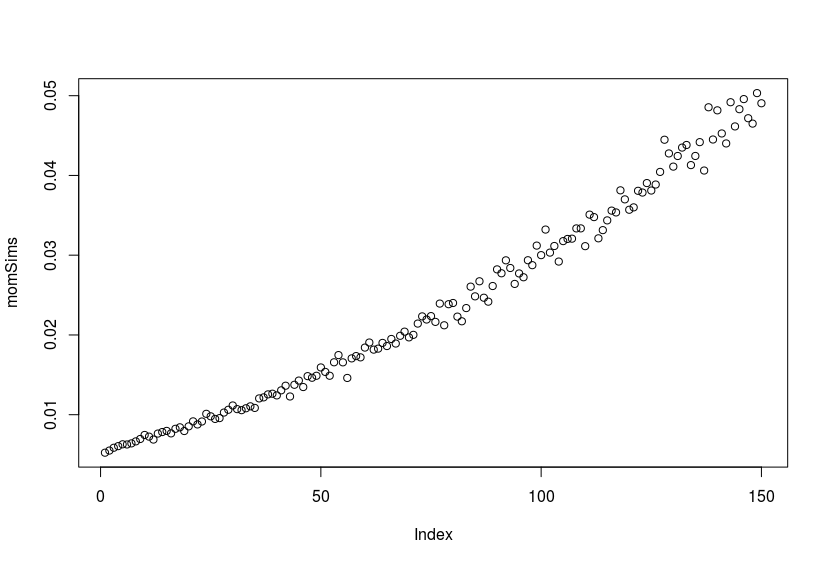
\includegraphics[scale=0.65]{plots/momSims.png}
\centering
\end{figure}
~\\
~\\

Error cuadratico medio de $B_{med}$
\begin{figure}[H]
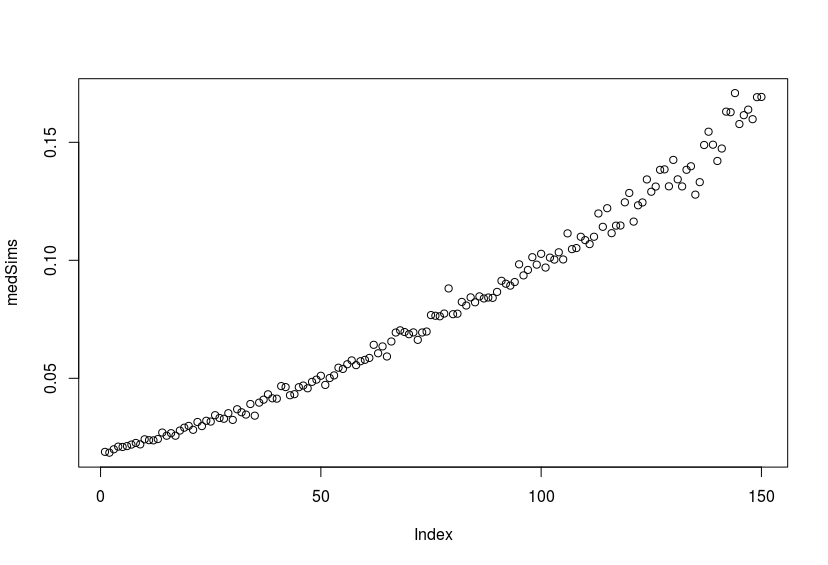
\includegraphics[scale=0.65]{plots/medSims.png}
\centering
\end{figure}
~\\
~\\

Error cuadratico medio de $B_{mv}$
\begin{figure}[H]
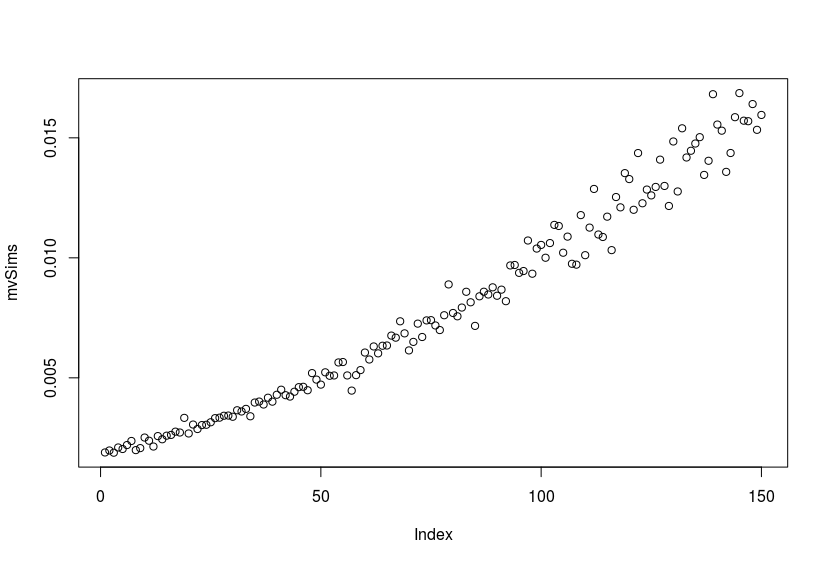
\includegraphics[scale=0.65]{plots/mvSims.png}
\centering
\end{figure}
~\\
~\\
Como puede eobservarse la magnitud del error es menor en el estimador de maxima verosimilitud, $B_{mv}$, que en los otros dos. Siendo el mestimador $B_{med}$ el que peor aproxima. Notar que si bien los datos en el grafico de $B_{mv}$ se ven mas dispersos, esto es asi gracias a que la escala vertical es menor, dado que el error lo es.
Respondiendo a la pregunta del enunciado, bajo esta medida, el estimador $B_{mv}$ funciona mejor que los otros dos, por lo cual elegiria ese.

\end{subsection}
\end{section}
\newpage




\begin{section}{Ejercicio 6}
Realizar un grafico de los ECM con b = 1 y n = 15, 30, 50, 100, 150, 200 ¿Que observa? ¿Que
estimador elige? ¿Que sospecha sobre la consistencia de los estimadores?

\begin{subsection}{Implementacion}


Se utiliza el siguiente codigo para generar los vectores.
\begin{verbatim}
b = 1;
ni = double();
ni <- c(15, 30, 50, 100, 150, 200);
niLen = 6;
momSims = double();
medSims = double();
mvSims = double();

for(i in 1:niLen){
	momSims[i] <- simulacion_mom(b,ni[i]);
	medSims[i] <- simulacion_med(b,ni[i]);
	mvSims[i] <- simulacion_mv(b,ni[i]);
}

\end{verbatim}

Y luego creamos los graficos compuestos con sl siguiente codigo:

\begin{verbatim}

> plot(ni, momSims, ylim=c(0,0.030))
> points(ni, medSims , col="red")
> points(ni, mvSims , col="green")
> 

\end{verbatim}

Se obtiene el siguiente grafico, donde los puntos de color negro son los de $B_{mom}$, los de color rojo los de $B_{med}$, y los de color verde los de $B_{mv}$.


Error cuadratico medio de $B_{mom}$
\begin{figure}[H]
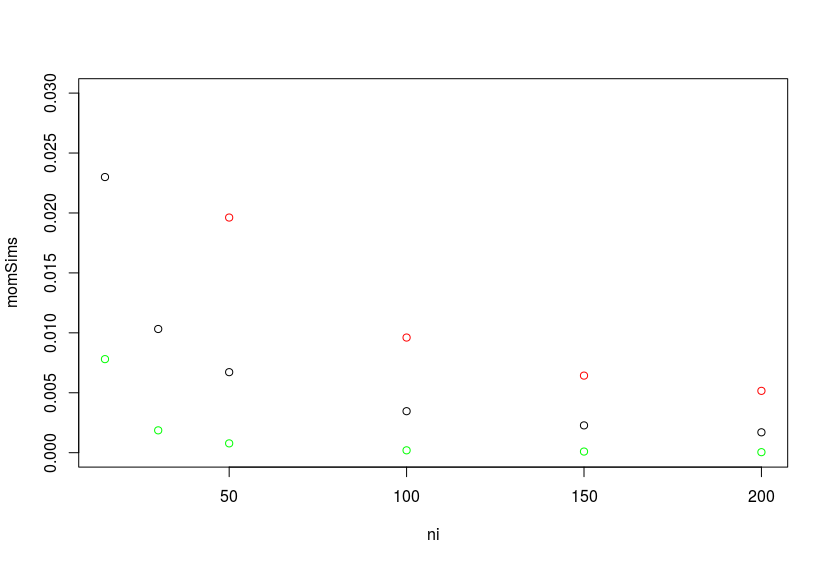
\includegraphics[scale=0.65]{plots/combNPlot.png}
\centering
\end{figure}
~\\
~\\



Nuevamente se observa una convergencia mas rapida para el estimador de maxima verosimilitud. Ademas, en cuanto a la consistencia, el unico estimador que converge al valor real, al menos con $n<200$, es el de maxima verosimilitud, con lo cual es el unico que parece consistente.
\end{subsection}
\end{section}
\newpage




\begin{section}{Ejercicio 8}
Calcular los estimadores en la siguiente muestra. ¿Observa algo extraño? ¿a que cree que se
debe? \\
~\\
0,917 0,247 0,384 0,530 0,798 0,912 0,096 0,684 0,394 20,1 0,769 0,137 0,352 0,332 0,670

\begin{subsection}{Implementacion}


Se utiliza el siguiente codigo para generar los vectores.
\begin{verbatim}

> vals = double();
> vals <- c(0.917, 0.247, 0.384, 0.530, 0.798, 0.912, 0.096, 0.684, 0.394, 20.1, 0.769, 0.137, 0.352, 0.332, 0.670)
> Rmed = Bmed(vals)
> Rmom = Bmom(vals)
> Rmv = Bmv(vals)
> print(Rmom)
[1] 3.642933
> print(Rmv)
[1] 20.1
> print(Rmed)
[1] 0.192
\end{verbatim}
Los resultados de los estimadores son (Bmom, Bmed, Bmv) = (3.642933, 0.192, 20.1). Es esperable que esto suceda ya que el estimador $B_{mv}$, estima utilizando el maximo. Si este fuera un outlier resultante de un error de medicion, nos estaria dando un muy mal resultado. Lo que esto nos dice es que este metodo es mas sensible a errores de medicion.


\end{subsection}
\end{section}
\newpage




\begin{section}{Ejercicio 4}
Aproximar sesgo, varianza y error cuadrático medio para los estimadores bajo el siguiente
escenario con datos atípicos:
Una muestra uniforme con $b = 1$ y $n = 15$ que con probabilidad $p = 0,05$ un elemento de la
muestra viene multiplicado por $100$ (coma corrida dos lugares a la derecha). ¿Que estimador
prefiere en este escenario?
Aclarción: Para generar una muestra en estas condiciones basta generar una muestra como
antes y luego decidir con probabilidad $ = 0,05$ multiplicar por $100$ al primer elemento de la
muestra.

\begin{subsection}{Implementacion}



\begin{verbatim}
	b = 1;
	n = 15;
	nrep = 2000;
	Bmoms = double()
	Bmeds = double()
	Bmvs = double()
	X = double()
	p = 0.05;
	acumP = 0;
	for (i in 1:nrep){
		acumP = acumP+p;

		X = runif(n, 0.0, b);
		if(acumP >= 1){
			acumP = 0;
			X[1] = X[1]*100;
		}
		Bmoms[i] <- Bmom(X);
		Bmeds[i] <- Bmed(X);
		Bmvs[i] <- Bmv(X);
	}
	momMean = mean(Bmoms);
	medMean = mean(Bmeds);
	mvMean = mean(Bmvs);

	momErr = abs(b-momMean);
	medErr = abs(b-medMean);
	mvErr = abs(b-mvMean);

\end{verbatim}
Los resultados conseguidos son los siguientes:

\begin{verbatim}

> print(momErr)
[1] 0.3071968
> print(medErr)
[1] 0.01177621
> print(mvErr)
[1] 2.20998
> 


\end{verbatim}
Aquí vemos que  (momErr, medErr, mvErr) = (0.3071968, 0.01177621, 2.20998).\\
recordemos que para una muestra uniforme, los resultados habian sido (momErr, medErr, mvErr) = (0.0002888454, 0.1260778, 0.06227115).\\
Sucede algo parecido a lo visto en el punto anterior. El hecho de que hjaya un outlier, perjudica la medida del estimador de maxima verosimilitud (en caso de ser un error).

Las varianzas muestrales de los estimadores son las siguientes:

\begin{verbatim}

> momVar = var(Bmoms)
> medVar = var(Bmeds)
> mvVar = var(Bmvs)
> print(momVar)
[1] 2.58347
> print(medVar)
[1] 0.3396885
> print(mvVar)
[1] 142.4497
> 

\end{verbatim}

La aproximacion obtenida para varianza da: \\
(momVar, medVar, mvVar) = (2.58347, 0.3396885, 142.4497)\\
Recordemos que los valores para muestras uniformes eran:\\
(momVar, medVar, mvVar) = (0.02233229, 0.05594595, 0.003525818)\\
Nuevamente vemos como el estimador de maxima verosimilitud es el mas afectado por estos nuevos valores.
Extrañamente, la varianza en el estimador de momentos se redujo.



Se utilizará esta formula de la aproximacion del ECM como antes:

\begin{verbatim}
> ECMBmom = momVar + (momErr^2);
> ECMBmed = medVar + (medErr^2);
> ECMBmv  = mvVar + (mvErr^2);
> print(ECMBmom)
[1] 2.677839
> print(ECMBmed)
[1] 0.3398272
> print(ECMBmv)
[1] 147.3337
> 
\end{verbatim}
~\\
Se obtiene así:\\
(ECMBmom, ECMBmed, ECMBmv) = (2.677839, 0.3398272, 147.3337)\\
~\\
Siendo los valores anteriores:\\
 (ECMBmom, ECMBmed, ECMBmv) = (0.02233238, 0.07184158, 0.007403514).\\
 ~\\
En este caso vuelve a observarse como cambia el valor en $B_{mv}$. Cabe preguntarse que estimador es mejor para este caso.
La respuesta es que si estamos seguros de que tpodas nuestras mediciones fueron realizadas correctamente, $B_{mv}$ es capaz de utilizar estos datos que parecen outliers para dar una mejor respuesta, pero en el caso general, en el que se espera que hayan errores de medicion, esta estimador es demasiado sensible a outliers. En este caso el estimador que mejor se comporta es aquel que menos utiliza la informacion de los outliers, es decir $B_{med}$. Esto puede verse reflejado en su menor error cuadratico medio.

\end{subsection}
\end{section}
\end{document}
